\begin{solution}
\begin{enumerate}

\item {[5 points]}
We can use the MATLAB code:

\lstinputlisting{HW1a.m}

to compute that
\[
a_n=\frac{-8\sin^2\left(\frac{n\pi}{2}\right)}{\sin\left(2n\pi\right)-2n\pi}.
\]
\\
\item {[5 points]}
If $n$ is an integer then $\sin\left(2n\pi\right)=0$ and therefore
\[
a_n=\frac{-8\sin^2\left(\frac{n\pi}{2}\right)}{-2n\pi}=\frac{4\sin^2\left(\frac{n\pi}{2}\right)}{\pi n}.
\]
\\
\item {[5 points]}
Now,
\[
\sin^2\left(\frac{n\pi}{2}\right)=\left\{\begin{array}{ll}
\displaystyle{1}, & \mbox{if }n\mbox{ is odd;}
\\
0, & \mbox{if }n\mbox{ is even.}
\end{array}\right.
\]
Consequently,
\[
a_n=\left\{\begin{array}{ll}
\displaystyle{\frac{4}{n\pi}}, & \mbox{if }n\mbox{ is odd;}
\\
0, & \mbox{if }n\mbox{ is even.}
\end{array}\right.
\]
\\
\item {[10 points]}
We can use the MATLAB code:

\lstinputlisting{HW1d.m}

to produce the plot:
\begin{center}
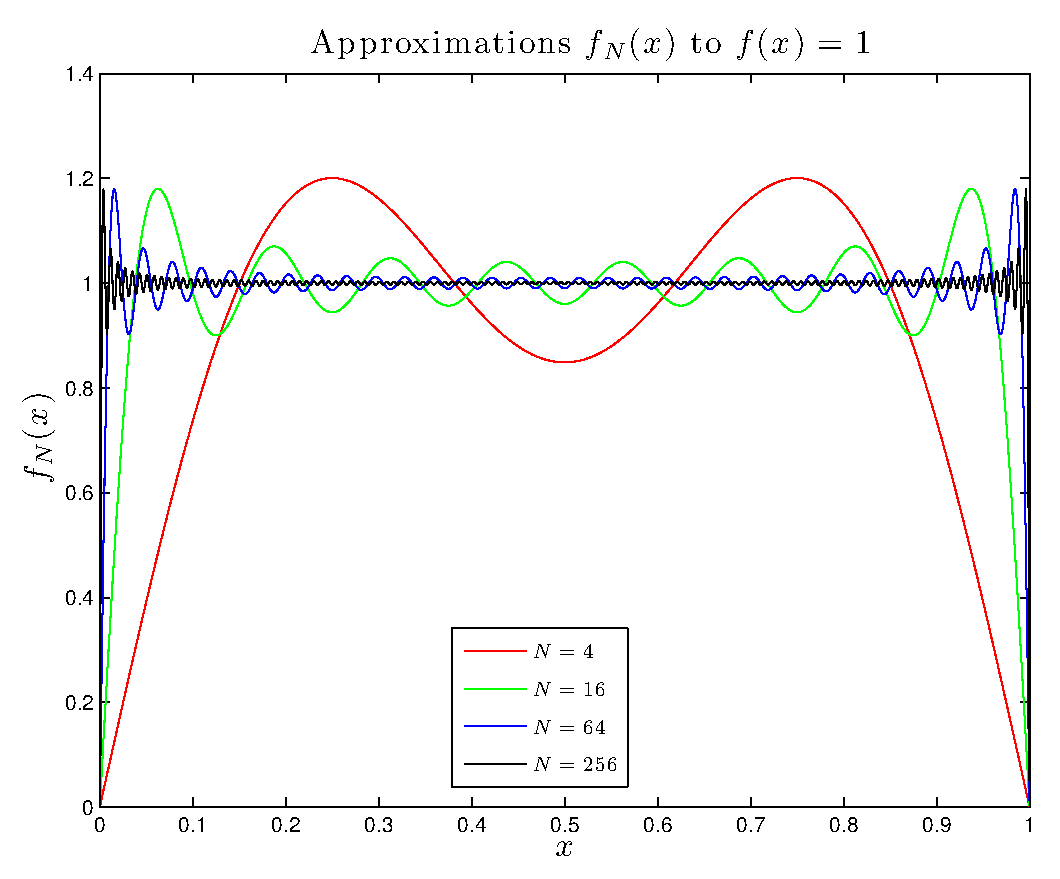
\includegraphics[scale=0.7]{hw1d.eps}
\end{center}
\end{enumerate}
\end{solution}